\documentclass[12pt]{article}

\usepackage{amsmath}
\usepackage{graphicx}
\usepackage{geometry}
\usepackage{setspace}
\usepackage{caption}

\geometry{margin=1in}
\onehalfspacing

\title{Emergent Scale-Invariance in the Bak--Tang--Wiesenfeld Sandpile Model: \\ 
A Computational Study of Self-Organized Criticality}

\author{
Ashwitha Rathod \\ 
Entry Number: 2022CH11475
}

\date{April 2026}

\begin{document}

\maketitle

\begin{abstract}

Many natural and engineered systems exhibit complex behaviour arising from interactions among many individual components. One of the most important concepts developed to explain such behaviour is self-organized criticality. Systems exhibiting this phenomenon naturally evolve toward a critical state in which events of widely varying sizes occur. 

This project investigates the Bak--Tang--Wiesenfeld (BTW) sandpile model, one of the earliest and most influential models demonstrating self-organized criticality. A computational simulation of the model was implemented using Python in order to study avalanche dynamics generated by local redistribution rules. Avalanche size distributions were recorded and analyzed to understand the statistical behaviour of the system. The simulation results show that avalanche sizes follow a heavy-tailed distribution consistent with power-law behaviour, indicating scale invariance and critical dynamics. These observations illustrate how complex macroscopic patterns can emerge from simple microscopic rules and local interactions.

\end{abstract}

\section{Introduction}

Complexity science studies systems composed of many interacting components whose collective behaviour cannot be easily predicted from the properties of individual elements. Examples include ecosystems, neural networks, economic markets, traffic flows, and geological systems such as earthquakes. A defining characteristic of many complex systems is the emergence of large-scale structures and patterns arising from simple local interactions.

One of the most significant discoveries in complexity science is the concept of \textit{self-organized criticality} (SOC). In systems exhibiting SOC, the system naturally evolves toward a critical state where disturbances can generate cascades of events across many different scales. Unlike traditional critical phenomena in physics, which require careful tuning of parameters, self-organized critical systems reach the critical state automatically.

The Bak--Tang--Wiesenfeld sandpile model, introduced in 1987, provides a simple yet powerful framework for studying self-organized criticality. Despite its simplicity, the model captures fundamental characteristics observed in many real-world systems, including avalanche dynamics, scale invariance, and emergent global behaviour.

The objective of this project is to study the behaviour of the sandpile model through computational simulation and analyze the statistical distribution of avalanche sizes generated within the system.

\section{The Sandpile Model as a Complex System}

The sandpile model represents a system in which local interactions between neighbouring sites produce complex global behaviour. The system consists of a two-dimensional lattice grid in which each site stores an integer number representing the height of sand grains accumulated at that location.

One of the reasons the sandpile model is widely studied in complexity science is that it demonstrates several defining properties of complex systems. First, the model involves a large number of interacting components arranged in a network-like structure. Each lattice site interacts with its neighbouring sites through redistribution of sand grains.

Second, the model exhibits nonlinear dynamics. A single grain of sand may have no observable effect, or it may trigger a large cascade of toppling events depending on the state of the surrounding lattice.

Third, the model generates emergent behaviour. Although the rules governing the system are extremely simple, the resulting avalanche dynamics display rich statistical patterns.

Finally, the system spontaneously evolves toward a critical state without external tuning of parameters. This self-organization toward a critical point is the defining feature of self-organized criticality.

\section{System Dynamics: Noise, Connectivity, and Avalanche Formation}

The dynamics of the sandpile system are driven by three key mechanisms: external perturbations, local connectivity between sites, and cascading avalanche events.

The driving mechanism of the system can be interpreted as a form of stochastic noise. At each simulation step, a grain of sand is added to a randomly selected location on the lattice. This continuous random input gradually increases the overall height of the sandpile and pushes the system toward instability.

Connectivity between sites determines how disturbances propagate through the system. In the model used in this study, each lattice site interacts with its four nearest neighbours: up, down, left, and right. This neighbourhood structure is often referred to as a von Neumann neighbourhood. The connectivity of the lattice forms the pathway through which toppling events can propagate.

Avalanches occur when the number of grains at a site exceeds a critical threshold. In the classical sandpile model, the threshold is four grains. When a site becomes unstable, it topples and redistributes one grain to each of its neighbouring sites. This redistribution may cause neighbouring sites to exceed the threshold as well, producing a cascade of further toppling events.

The resulting chain reaction is known as an avalanche. Avalanches can involve only a few topplings or can spread across large portions of the lattice depending on the configuration of the system.

\section{Computational Simulation}

A computational simulation of the sandpile model was implemented using the Python programming language. The simulation represents the lattice as a two-dimensional grid in which each cell stores the number of grains present at that location.

The simulation begins with an initially empty lattice. At each iteration, a grain is added to a randomly selected lattice site. If the number of grains at that site reaches the critical threshold, a toppling event occurs and grains are redistributed to neighbouring sites.

The system is then checked for further unstable sites. If additional sites exceed the threshold, further toppling events occur until the system becomes stable again. The total number of topplings that occur during this cascade is recorded as the avalanche size.

The simulation was run for a large number of iterations in order to collect sufficient statistical data on avalanche events. The avalanche sizes generated during the simulation were stored and later analyzed to study the statistical properties of the system.

\section{Avalanche Size Distribution}

The recorded avalanche sizes provide insight into the statistical behaviour of the system. In particular, the distribution of avalanche sizes reveals important information about the presence of critical dynamics.

Figure~\ref{fig:avalanche} shows the frequency distribution of avalanche sizes obtained from the simulation.

\begin{figure}[h]
\centering
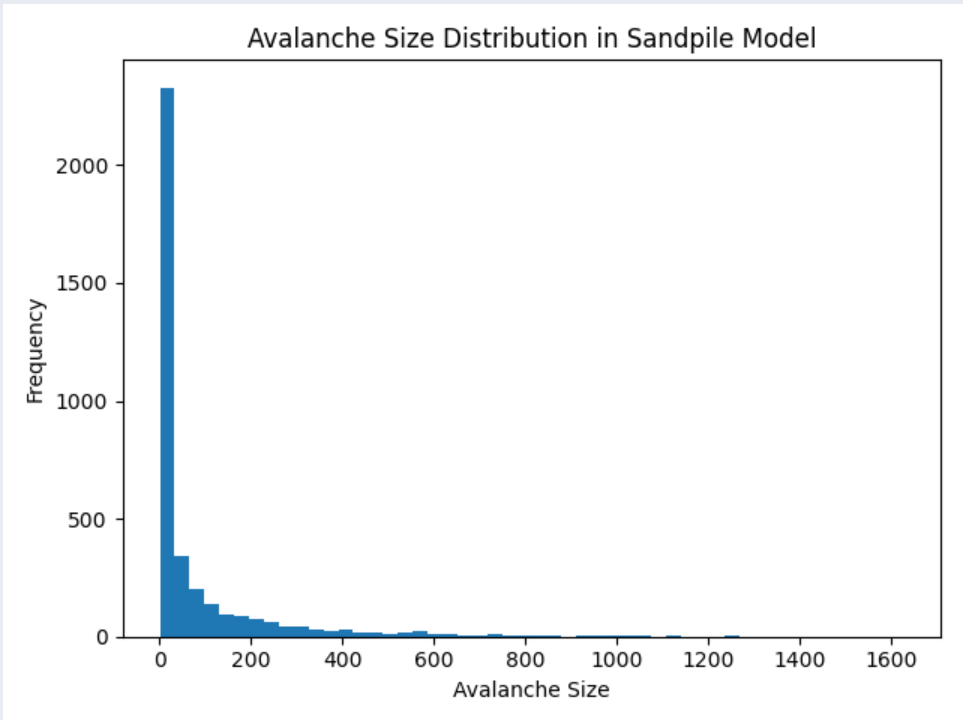
\includegraphics[width=0.85\textwidth]{avalanche_distribution.png}
\caption{Distribution of avalanche sizes obtained from the sandpile simulation. The histogram shows that small avalanches occur frequently, while large avalanches occur less often.}
\label{fig:avalanche}
\end{figure}

The histogram demonstrates that the majority of avalanche events are small, while large avalanches occur relatively rarely. However, large events still occur occasionally, indicating that the system does not possess a characteristic avalanche size.

This behaviour is consistent with a power-law distribution of avalanche sizes of the form

\[
P(s) \propto s^{-\tau}
\]

where $s$ represents the avalanche size and $\tau$ is the scaling exponent. Power-law behaviour is a hallmark of systems operating at criticality and indicates scale-invariant dynamics.

The connectivity of the lattice plays a crucial role in shaping the avalanche distribution. Because each site is connected to four neighbouring sites, disturbances can propagate across the lattice and produce cascades spanning multiple spatial scales.

\section{Self-Organized Critical Behaviour}

The sandpile model naturally evolves toward a critical state in which the system remains poised between stability and instability. In this state, the addition of a single grain of sand may trigger avalanches of widely varying sizes.

The absence of a characteristic avalanche scale indicates that the system operates near a critical point. Unlike traditional critical phenomena in statistical physics, which require careful tuning of parameters such as temperature or pressure, the sandpile model reaches this critical state automatically through its internal dynamics.

This behaviour illustrates the concept of self-organized criticality. Systems exhibiting SOC continuously reorganize themselves so that the system remains close to a critical threshold. As a result, disturbances can propagate through the system in the form of avalanches spanning many different scales.

Similar behaviour has been observed in a variety of real-world systems including earthquakes, forest fires, landslides, and financial market fluctuations.

\section{Conclusion}

This study investigated the dynamics of the Bak--Tang--Wiesenfeld sandpile model through computational simulation. The model provides a simple yet powerful framework for understanding how complex behaviour can arise from local interactions.

The simulation results demonstrate that the sandpile system generates avalanche events across a wide range of sizes. The observed avalanche size distribution exhibits heavy-tailed behaviour consistent with power-law scaling, indicating scale-invariant dynamics.

These results illustrate how the sandpile model naturally evolves toward a self-organized critical state. The emergence of critical behaviour without external tuning highlights the fundamental principles of complexity science and demonstrates how simple rules can generate rich collective dynamics.
\section{Prompts Used During the Preparation of This Project}

The following prompts were used to guide the development of the simulation code, analysis, and manuscript preparation:

\begin{itemize}

\item Explain the concept of self-organized criticality in the Bak–Tang–Wiesenfeld sandpile model.

\item Describe why the sandpile model is a suitable example for studying complexity science.

\item Generate Python code to simulate the Bak–Tang–Wiesenfeld sandpile model on a two-dimensional lattice.

\item Explain how avalanches occur in the sandpile model and how they propagate through neighbouring sites.

\item Explain the roles of noise, avalanche dynamics, and connectivity in complex systems.

\item How can avalanche size distributions be analyzed in a sandpile simulation?

\item Write a research-style LaTeX report describing the sandpile model simulation and its statistical behaviour.

\end{itemize}
\section{Acknowledgments}

The computational simulations in this project were implemented using Python with the NumPy and Matplotlib libraries. The conceptual framework of self-organized criticality was originally introduced by Per Bak, Chao Tang, and Kurt Wiesenfeld.

\end{document}